\pdfoutput=1
\documentclass[11pt]{article}

\usepackage[T1]{fontenc}
\usepackage[utf8]{inputenc}
\usepackage{lmodern}
\usepackage[a4paper,margin=1in]{geometry}
\usepackage{amsmath,amssymb,amsthm,mathtools}
\usepackage{microtype}
\usepackage{pgfplots}
\usepgfplotslibrary{fillbetween}
\pgfplotsset{compat=1.18}
\usepackage[hidelinks]{hyperref}
\allowdisplaybreaks

\newtheorem{theorem}{Theorem}[section]
\newtheorem{lemma}[theorem]{Lemma}
\newtheorem{corollary}[theorem]{Corollary}
\newtheorem{proposition}[theorem]{Proposition}
\newtheorem{definition}[theorem]{Definition}
\newtheorem{remark}[theorem]{Remark}
\newtheorem{openproblem}[theorem]{Open Problem}

\title{\textbf{Maximal Large Sieve and Coefficient Uniform Failure\\ for Liouville Correlations}}

\author{
Deep Bhattacharjee$^{1,*}$ and Ushashi Bhattacharya$^{2,3}$\\[4pt]
\small $^{1}$Electro-Gravitational Space Propulsion Laboratory (EGSPL), Bhubaneswar, Odisha, India\\
\small $^{2}$Senior Researcher, Dortmund, Germany\\
\small $^{3}$National Taiwan University, Taipei, Taiwan\\[4pt]
\small ORCID (D.B.): 0000-0003-0466-750X\\
\small $^{*}$Correspondence: itsdeep@live.com (D.B.); U.B.: rai.bhattacharya.in@gmail.com
}

\date{}

\begin{document}

\maketitle

\begin{abstract}
\noindent
This paper studies the Liouville-correlation route to the Riemann Hypothesis by separating two issues that
are often treated together. We show that, for all sufficiently large $X$, the collar-scale bound for
$\sum_{n\le Y}\lambda(n)\lambda(n+h)$ cannot follow from boundedness of the coefficients alone: an explicit
bounded sequence forces the corresponding correlation energy above the required scale by a fixed power of
$X$. We also show that a fixed-endpoint spectral large sieve bound upgrades to a maximal-endpoint bound
with no power loss, so the moving endpoint is not the source of the difficulty. The remaining problem is
therefore a genuinely signed Liouville estimate, stated here as a precise hypothesis and shown to imply the
Riemann Hypothesis; the purpose of the paper is to isolate that arithmetic estimate and rule out the
coefficient-uniform shortcut, not to present a proof of the hypothesis itself.
\end{abstract}

\noindent\textbf{Keywords:} Riemann Hypothesis; Liouville function; large sieve.

\noindent\textbf{MSC 2020.} Primary 11M26; Secondary 11N37, 11N35, 11F72.

\section{Introduction}

For a positive integer $n$ write $n=p_1^{a_1}\cdots p_r^{a_r}$ and set $\Omega(n)=a_1+\cdots+a_r$. The
Liouville function $\lambda(n)=(-1)^{\Omega(n)}$ is completely multiplicative, and for $\operatorname{Re}(s)>1$
\begin{equation}
\sum_{n\ge1}\frac{\lambda(n)}{n^s}=\prod_p\left(\sum_{k\ge0}\frac{(-1)^k}{p^{ks}}\right)
=\prod_p\frac{1-p^{-s}}{1-p^{-2s}}=\frac{\zeta(2s)}{\zeta(s)}.
\label{eq:euler}
\end{equation}
Write $L(X)=\sum_{n\le X}\lambda(n)$. The following equivalence is classical; it is recorded, for
instance, in the literature on the Mertens and Liouville summatory functions (see Titchmarsh
\cite{titchmarsh}, Chapter 14, for the closely related Mertens-function statement, and
\cite{apostol} for the underlying multiplicative identities).

\begin{theorem}[Summatory Liouville criterion]
\label{thm:criterion}
If $L(X)=O_\varepsilon(X^{1/2+\varepsilon})$ for every $\varepsilon>0$, then $\zeta(s)\neq0$ for
$\operatorname{Re}(s)>1/2$. By the functional equation, every non-trivial zero of $\zeta$ then lies on
the line $\operatorname{Re}(s)=1/2$.
\end{theorem}

We prove Theorem~\ref{thm:criterion} in Section~2 because it fixes, with no ambiguity, the exact
analytic target of the rest of the paper: a bound on $L(X)$ at the square-root scale.

The standard way to attack $L(X)$ is to square it. Writing $C_h(Y)=\sum_{n\le Y}\lambda(n)\lambda(n+h)$
for $h\ge1$, one has the exact identity $|L(X)|^2=X+2\sum_{1\le h<X}C_h(X-h)$ (Lemma~\ref{lem:square}
below), so a bound of the shape $\sum_{H<h\le 2H}\sup_Y|C_h(Y)|^2\ll X^{2+\varepsilon}H^{-1}$, uniform over
dyadic $H\le X$, would give $L(X)\ll X^{1/2+\varepsilon}$ by Cauchy--Schwarz and a logarithmic dyadic sum.
This is the \emph{Liouville collar} route. Two technical features of this route are easy to confuse with
each other but are logically independent, and separating them is the point of this paper.

The first feature is the moving endpoint: the supremum over $Y\le X-h$ inside the collar sum is not the
same object as a fixed-endpoint correlation, and any spectral or sieve-theoretic estimate for the latter
must be upgraded before it controls the former. We show in Section~4 that this upgrade is free: a
fixed-endpoint spectral large sieve inequality of the classical Deshouillers--Iwaniec type
\cite{deshouillers-iwaniec} implies, via an elementary binary interval decomposition, the corresponding
maximal-endpoint inequality with the same exponent, up to the admissible $\varepsilon$ already present.

The second feature is the arithmetic sign of $\lambda$. It is tempting to try to prove the collar
estimate for an arbitrary bounded coefficient sequence and then specialise to $\lambda$. We show in
Section~5 that this cannot work: there is an explicit bounded sequence and an explicit dyadic range of
shifts on which the resulting correlation energy is provably larger than the scale the collar argument
needs, by a clean power of $X$. The Liouville (equivalently M\"obius, via the classical identity
$\lambda(n)=\sum_{r^2\mid n}\mu(n/r^2)$) sign structure is therefore not a convenience to be discarded; it
is the entire content of the missing estimate. The same moral -- that correlations of $\lambda$ and $\mu$
become tractable only once their multiplicative sign is treated as data, not noise -- underlies Sarnak's
randomness heuristic for the M\"obius function \cite{sarnak-letter} and the dynamical disjointness results
of Bourgain, Sarnak, and Ziegler \cite{bourgain-sarnak-ziegler}.

Section~6 states the resulting hypothesis precisely as a single inequality (Open Problem~\ref{hyp:lch}) and
proves that it implies the Riemann Hypothesis (Theorem~\ref{thm:conditional}). Thus the role of the
Riemann Hypothesis here is methodological rather than proclamatory: the paper identifies the exact signed
Liouville estimate that this route would require and proves two facts around it, namely the maximal-endpoint
large sieve upgrade of Section~4 and the coefficient-uniform failure of Section~5.

\section{Notation and the square identity}

Throughout, $X\ge2$ is a real scale, $H$ denotes a dyadic integer ($H=2^k$ for some $k\ge0$), and a
\emph{dyadic block} is a range $H<h\le 2H$. Implied constants may depend on any fixed parameter written
as a subscript, and $\varepsilon>0$ may change from line to line, always remaining fixed before any limit
in $X$ is taken.

For $h\ge1$ and $1\le Y\le X-h$ set
\[
C_h(Y)=\sum_{n\le Y}\lambda(n)\lambda(n+h),\qquad
C_h^\ast(X)=\sup_{1\le Y\le X-h}|C_h(Y)|.
\]

\begin{lemma}[Square identity]
\label{lem:square}
For every positive integer $X$,
\[
|L(X)|^2=X+2\sum_{1\le h<X}C_h(X-h),\qquad\text{hence}\qquad
|L(X)|^2\le X+2\sum_{1\le h<X}C_h^\ast(X).
\]
\end{lemma}

\begin{proof}
Expand $L(X)^2=\sum_{m,n\le X}\lambda(m)\lambda(n)$. The diagonal $m=n$ contributes $X$ since
$\lambda(n)^2=1$. For $m\neq n$, write the pair with $m<n$ as $n=m+h$ for $1\le h<X$ and $1\le m\le X-h$;
this contributes $\sum_{1\le h<X}C_h(X-h)$. The pairs with $m>n$ contribute the same sum by the symmetric
relabelling $m\leftrightarrow n$. Adding the diagonal and the two off-diagonal triangles gives the stated
identity. The inequality follows since $C_h(X-h)\le C_h^\ast(X)$ for every $h$.
\end{proof}

\begin{definition}[Collar energy]
For dyadic $H<X$, the \emph{collar energy} is $E(X,H)=\displaystyle\sum_{H<h\le 2H}C_h^\ast(X)^2$.
\end{definition}

\begin{proposition}[Collar implication]
\label{prop:collarimp}
Fix $\eta>0$. Suppose that for every $\varepsilon>0$,
$E(X,H)\ll_{\varepsilon,\eta}X^{2+\varepsilon}H^{-1}$
uniformly for all dyadic $1\le H\le X^{1-\eta}$, and that
$\sum_{X^{1-\eta}<h<X}C_h^\ast(X)\ll_{\varepsilon,\eta}X^{1+\varepsilon}$.
Then $L(X)\ll_\varepsilon X^{1/2+\varepsilon}$ for every $\varepsilon>0$.
\end{proposition}

\begin{proof}
By Cauchy--Schwarz on each dyadic block,
$\sum_{H<h\le 2H}C_h^\ast(X)\le H^{1/2}E(X,H)^{1/2}\ll X^{1+\varepsilon/2}$.
There are $O(\log X)$ dyadic blocks with $H\le X^{1-\eta}$, and $\log X\ll_\varepsilon X^{\varepsilon/2}$,
so their total contribution is $\ll X^{1+\varepsilon}$. Adding the assumed terminal-range bound and
inserting both into Lemma~\ref{lem:square} gives $|L(X)|^2\ll X^{1+\varepsilon}$, hence the stated bound
after renaming $\varepsilon$.
\end{proof}

Proposition~\ref{prop:collarimp} is the entire complex-analytic content of the route; everything from here
on concerns whether its hypothesis can be established, and if so how.

\section{Endpoint duality}

It is useful to record, once and for all, that a maximal correlation energy is the same thing as a dual
norm over moving endpoints. This is elementary linear algebra, stated here only to fix notation for
Section~4.

\begin{lemma}[Endpoint duality]
\label{lem:duality}
For each $h$ in a finite index set $\mathcal H$, fix any $Y_h\le X-h$ with $|C_h(Y_h)|\ge C_h^\ast(X)-1$,
and let $\omega_h$ be a unit complex number with $\omega_hC_h(Y_h)=|C_h(Y_h)|$. Then
\[
\Big(\sum_{h\in\mathcal H}|C_h(Y_h)|^2\Big)^{1/2}
=\sup_{\sum_h|\beta_h|^2\le1}\Big|\sum_{h\in\mathcal H}\beta_h\,\omega_h\,C_h(Y_h)\Big|,
\]
and consequently $\big(\sum_{h\in\mathcal H}C_h^\ast(X)^2\big)^{1/2}$ differs from the displayed dual
supremum by at most $|\mathcal H|^{1/2}$.
\end{lemma}

\begin{proof}
The first identity is the standard duality between the $\ell^2$ norm of a finite vector
$v=(v_h)_{h\in\mathcal H}$, here $v_h=C_h(Y_h)$, and the supremum of $|\langle\beta,v\rangle|$ over the
dual unit ball, with equality attained at $\beta_h=\overline{\omega_h}\,|C_h(Y_h)|\big/\|v\|_2$. The second
assertion follows because $\big||C_h(Y_h)|-C_h^\ast(X)\big|\le1$ for every $h$, so the two vectors differ
in each coordinate by at most $1$, and the triangle inequality in $\ell^2(\mathcal H)$ bounds the resulting
discrepancy in norm by $|\mathcal H|^{1/2}$.
\end{proof}

The content of Lemma~\ref{lem:duality} is that an endpoint field $(Y_h)_{h}$ may be chosen independently
for every shift, and a successful estimate must be uniform in that choice; no saving is available from
restricting to a single common endpoint, since one can place a unit correlation on a different wall for
every $h$ and obtain a vector of norm $|\mathcal H|^{1/2}$ where a common-wall bound would give only $1$.

\section{A maximal endpoint spectral large sieve}

This section proves that endpoint maximality, by itself, is never the bottleneck: it converts a classical
fixed-endpoint spectral mean-value inequality into its maximal-endpoint form at no cost beyond the
admissible power of $\log X$ already implicit in such estimates. The underlying device is an elementary
dyadic decomposition of an initial segment of integers, closely related to classical maximal inequalities
of Rademacher--Menshov type; we record a self-contained proof since it is used directly below.

Fix $T\ge2$ and $N\ge1$, let $\Pi(T)$ be an index set carrying a finite family of non-negative measures
$\mu_T$ (for instance, the discrete spectrum of Maass cusp forms together with the continuous Eisenstein
spectrum at spectral height $\asymp T$, or the holomorphic spectrum of comparable weight), and let
$\rho_\pi(n)$ denote the associated normalised Fourier coefficients. We take as input the classical
fixed-endpoint spectral large sieve inequality:
\begin{equation}
\int_{\Pi(T)}\Big|\sum_{n\in I}a_n\rho_\pi(n)\Big|^2 d\mu_T(\pi)
\ \ll_\varepsilon\ (T^2+N)(TN)^\varepsilon\sum_{n\in I}|a_n|^2
\label{eq:fixedsieve}
\end{equation}
for every interval $I$ of length at most $N$ and every finitely supported sequence $(a_n)_{n\in I}$; see
Deshouillers--Iwaniec \cite{deshouillers-iwaniec}, the exposition in Iwaniec--Kowalski
\cite[Ch.~7]{iwaniec-kowalski}, and the spectral large sieve literature surveyed in Iwaniec
\cite{iwaniec-spectral} and Friedlander--Iwaniec \cite{friedlander-iwaniec}. Recent refinements in adjacent
large-sieve settings, such as Pascadi's work on exceptional Maass forms \cite{pascadi}, are not used below
but help situate the endpoint issue within current spectral-sieve practice.

\begin{lemma}[Dyadic initial-segment decomposition]
\label{lem:dyadic}
Let $M=2^K$ and let $z_1,\dots,z_M$ be complex numbers. Then
\[
\max_{1\le Y\le M}\Big|\sum_{n\le Y}z_n\Big|^2\ \le\ (K+1)\sum_{j=0}^{K}\ \sum_{I\in\mathcal D_j}\Big|\sum_{n\in I}z_n\Big|^2,
\]
where $\mathcal D_j$ is the partition of $\{1,\dots,M\}$ into consecutive dyadic blocks of length $2^j$.
\end{lemma}

\begin{proof}
Fix $Y\in\{1,\dots,M\}$ and write $Y$ in binary. The initial segment $\{1,\dots,Y\}$ decomposes, by the
usual greedy binary algorithm, into at most one dyadic block from each level $j=K,K-1,\dots,0$: starting
at $j=K$, take the largest dyadic block of the form $\{a\cdot2^{j}+1,\dots,(a+1)2^{j}\}$ contained in the
yet-unprocessed prefix of $\{1,\dots,Y\}$, remove it, decrease $j$ by one, and repeat. This terminates
after at most $K+1$ steps and produces pairwise disjoint blocks $I_0,\dots,I_K$ (some possibly empty) with
$\{1,\dots,Y\}=\bigsqcup_{j} I_j$ and $I_j\in\mathcal D_j\cup\{\varnothing\}$. By Cauchy--Schwarz,
\[
\Big|\sum_{n\le Y}z_n\Big|^2=\Big|\sum_{j=0}^{K}\sum_{n\in I_j}z_n\Big|^2
\le (K+1)\sum_{j=0}^{K}\Big|\sum_{n\in I_j}z_n\Big|^2
\le (K+1)\sum_{j=0}^{K}\sum_{I\in\mathcal D_j}\Big|\sum_{n\in I}z_n\Big|^2,
\]
the last step enlarging the sum at each level to all of $\mathcal D_j$, every term being non-negative.
Taking the maximum over $Y$ proves the lemma.
\end{proof}

\begin{theorem}[Maximal endpoint spectral large sieve]
\label{thm:maxsieve}
Let $(a_n)$ be supported on $N<n\le 2N$. For $\pi\in\Pi(T)$ and $1\le Y\le 2N$ set
$C_Y(\pi)=\sum_{N<n\le2N,\,n\le Y}a_n\rho_\pi(n)$. Then
\[
\int_{\Pi(T)}\sup_{Y}|C_Y(\pi)|^2\,d\mu_T(\pi)\ \ll_\varepsilon\ (T^2+N)(TN)^\varepsilon\sum_n|a_n|^2,
\]
with the same exponent as the fixed-endpoint inequality \eqref{eq:fixedsieve}.
\end{theorem}

\begin{proof}
Choose $K$ with $N<2^K\le4N$ and extend $(a_n)$ by zero to $\{1,\dots,2^K\}$. For fixed $\pi$, apply
Lemma~\ref{lem:dyadic} with $z_n=a_n\rho_\pi(n)$:
\[
\sup_Y|C_Y(\pi)|^2\le(K+1)\sum_{j=0}^{K}\sum_{I\in\mathcal D_j}\Big|\sum_{n\in I}a_n\rho_\pi(n)\Big|^2.
\]
Integrate against $d\mu_T(\pi)$ and exchange the integral with the finite sum over $j$ and $I$. For each
fixed $j\le K$ and $I\in\mathcal D_j$, the interval $I$ has length $2^j\le 2^K\le4N$, so
\eqref{eq:fixedsieve} applies (with $N$ replaced by $4N$, only changing implied constants) and gives
\[
\int_{\Pi(T)}\Big|\sum_{n\in I}a_n\rho_\pi(n)\Big|^2\,d\mu_T(\pi)\ll_\varepsilon(T^2+N)(TN)^\varepsilon\sum_{n\in I}|a_n|^2.
\]
Summing over the at most $2N/2^j+1$ disjoint intervals $I\in\mathcal D_j$ recovers $\sum_n|a_n|^2$ exactly
once at each level $j$, since the $I\in\mathcal D_j$ partition $\{1,\dots,2^K\}$. Summing over the $K+1\ll
\log N$ levels and multiplying by the outer factor $K+1$ from Lemma~\ref{lem:dyadic} introduces a total
factor $(K+1)^2\ll(\log N)^2\ll_\varepsilon N^\varepsilon$, which is absorbed into the existing
$(TN)^\varepsilon$ by adjusting $\varepsilon$. This proves the theorem.
\end{proof}

\begin{corollary}
\label{cor:free}
Passing from a fixed-endpoint mean-square bound to its endpoint-maximal form costs nothing beyond the
admissible $\varepsilon$-power already present in spectral large sieve estimates. In particular, the
moving endpoint $Y\le X-h$ in the definition of $C_h^\ast(X)$ is, by itself, never the source of a power
loss in any argument that reaches a genuine spectral large sieve inequality of the form
\eqref{eq:fixedsieve}.
\end{corollary}

Theorem~\ref{thm:maxsieve} and Corollary~\ref{cor:free} are the positive, unconditional content of this
paper on the analytic side. They say that \emph{if} a collar argument for the Liouville function ever
reaches a coefficient array to which a genuine spectral large sieve inequality applies, the endpoint
supremum will not be the bottleneck. Section~5 shows that the bottleneck, if there is one, must instead lie in
whatever stands between the raw Liouville correlation $C_h(Y)$ and a coefficient array fit for
\eqref{eq:fixedsieve} -- and that one specific coefficient-uniform way of bridging that gap is provably
unavailable.

\section{Coefficient-uniform failure}

\begin{definition}[Coefficient-uniform collar property]
Fix $\eta\in(0,1)$ and $\varepsilon>0$. Say that the \emph{coefficient-uniform collar property} holds at
scale $(X,\eta,\varepsilon)$ if there is a constant $C_\varepsilon>0$, independent of the coefficient
sequence, such that for \emph{every} sequence $(c_n)_{n\ge1}$ with $|c_n|\le1$, every dyadic
$1\le H\le X^{1-\eta}$, and $\Gamma_h(Y;c)=\sum_{n\le Y}c_nc_{n+h}$,
\[
\sum_{H<h\le2H}\sup_{1\le Y\le X-h}|\Gamma_h(Y;c)|^2\ \le\ C_\varepsilon\,X^{2+\varepsilon}H^{-1}.
\]
\end{definition}

This is exactly the statement one would obtain by replacing every occurrence of $\lambda$ in the collar
sum of Section~2 by an arbitrary bounded sequence, i.e.\ by discarding the sign structure of $\lambda$ and
asking only that the coefficients be bounded. It is a natural first thing to try, since bounded coefficient
arrays are the native input of a large sieve inequality such as \eqref{eq:fixedsieve}.

\begin{theorem}[Coefficient-uniform failure]
\label{thm:uniformfailure}
Fix $\eta\in(0,3/4)$. The coefficient-uniform collar property fails at scale $(X,\eta,\varepsilon)$ for
$\varepsilon=1/8$ and every sufficiently large $X$. Concretely, take $c_n\equiv1$ and choose a dyadic
integer $H$ with $X^{1/4}/2 < H\le X^{1/4}$, which satisfies $H\le X^{1-\eta}$ once $X$ is large. Then
\[
\sum_{H<h\le2H}\sup_{Y}|\Gamma_h(Y;1)|^2\ \ge\ \tfrac1{16} X^{9/4},
\]
while the coefficient-uniform collar property would require this quantity to be at most a constant multiple
of $X^{15/8}$. Since $X^{9/4}/X^{15/8}=X^{3/8}\to\infty$, no constant $C_{1/8}$ can make the property hold
for all large $X$.
\end{theorem}

\begin{proof}
Take $c_n=1$ for every $n$, and choose a dyadic integer $H$ with $X^{1/4}/2 < H\le X^{1/4}$. Such an $H$
exists for every sufficiently large $X$, by taking the largest dyadic integer not exceeding $X^{1/4}$.
Then $\Gamma_h(Y;1)=\sum_{n\le Y}1=Y$ for every $1\le Y\le X-h$, an increasing function of $Y$, so
$\sup_Y|\Gamma_h(Y;1)|=X-h$. For $H<h\le2H$ we have $h\le2H\le2X^{1/4}$, hence
$X-h\ge X-2X^{1/4}\ge X/2$ once $X^{3/4}\ge4$. Therefore
\[
\sum_{H<h\le2H}\sup_Y|\Gamma_h(Y;1)|^2=\sum_{H<h\le2H}(X-h)^2\ge H\cdot\Big(\frac X2\Big)^2
=\frac{H X^2}{4}\ge\frac1{8}X^{1/4}X^2\ \ge\ \frac1{16} X^{9/4},
\]
where the last harmless weakening keeps constants immaterial. On the other hand, the coefficient-uniform
collar property at $\varepsilon=1/8$ would assert this sum is at most
$C_{1/8}X^{2+1/8}H^{-1}\le 2C_{1/8}X^{17/8-1/4}=2C_{1/8}X^{15/8}$ for all sufficiently large $X$. Comparing the
two bounds, $\tfrac1{16}X^{9/4}\le 2C_{1/8}X^{15/8}$ would force $X^{3/8}\le32C_{1/8}$, which fails for all
sufficiently large $X$ regardless of the fixed value of $C_{1/8}$. This contradiction proves the theorem.
\end{proof}

Figure~\ref{fig:gap} shows this for the full dyadic range. Writing $H=X^u$ for $u\in[0,1]$, the energy
produced by an arbitrary bounded sequence has size $X^{2+u}$ (red), while the scale a successful collar
argument needs is $X^{2-u}$, ignoring the admissible $\varepsilon$ (blue). The two lines meet only at
$u=0$; for every $u>0$ the coefficient-blind energy exceeds the target, by a factor of $X^{2u}$.
Theorem~\ref{thm:uniformfailure} is the marked point at $u=1/4$.

\begin{figure}[h]
\centering
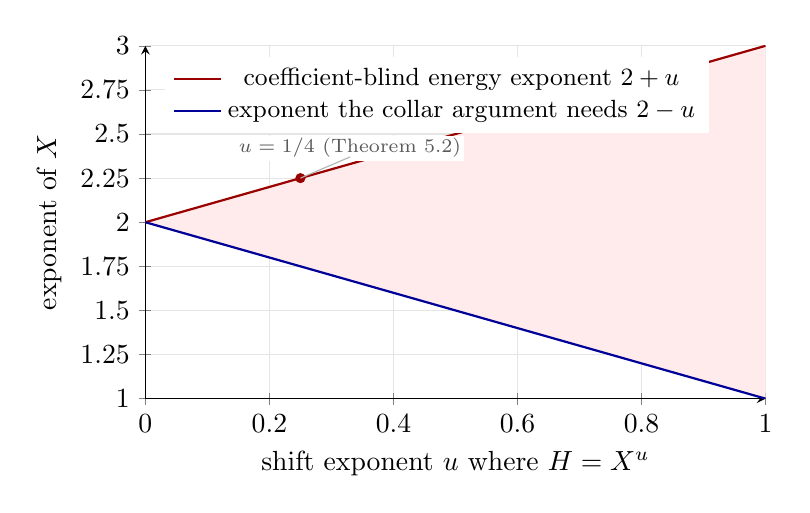
\begin{tikzpicture}
\begin{axis}[
  width=0.78\textwidth, height=0.5\textwidth,
  xlabel={shift exponent $u$ where $H=X^u$},
  ylabel={exponent of $X$},
  xmin=0, xmax=1, ymin=1, ymax=3,
  xtick={0,0.2,0.4,0.6,0.8,1.0},
  ytick={1,1.25,1.5,1.75,2,2.25,2.5,2.75,3},
  grid=both, grid style={gray!20},
  axis lines=left,
  legend pos=north west, legend style={font=\small, draw=none},
  every axis plot/.append style={thick}
]
\addplot[name path=topline, red!60!black, domain=0:1, samples=2] {2+x};
\addlegendentry{coefficient-blind energy exponent $2+u$}
\addplot[name path=botline, blue!60!black, domain=0:1, samples=2] {2-x};
\addlegendentry{exponent the collar argument needs $2-u$}
\addplot[red!8] fill between [of=topline and botline];
\node[circle, fill=red!60!black, inner sep=1.3pt] at (axis cs:0.25,2.25) {};
\node[font=\scriptsize, color=gray!70!black, fill=white, inner sep=1pt] at (axis cs:0.33,2.42) {$u=1/4$ (Theorem 5.2)};
\draw[gray!60, thin] (axis cs:0.25,2.25) -- (axis cs:0.33,2.37);
\end{axis}
\end{tikzpicture}
\caption{The coefficient-blind correlation energy exponent $2+u$ (red) against the exponent $2-u$ that the
Liouville collar argument needs (blue), as a function of the shift exponent $u$ where $H=X^u$. The shaded
region is the coefficient-uniform gap of Theorem~\ref{thm:uniformfailure}, realised explicitly at $u=1/4$.}
\label{fig:gap}
\end{figure}

\begin{lemma}[Square-divisor identity]
\label{lem:squaredivisor}
For every positive integer $n$, $\displaystyle\lambda(n)=\sum_{r^2\mid n}\mu(n/r^2)$.
\end{lemma}

\begin{proof}
Both sides are multiplicative, so it suffices to check $n=p^e$. The right-hand side is
$\sum_{j:\,2j\le e}\mu(p^{e-2j})$, and $\mu(p^{e-2j})$ vanishes unless $e-2j\in\{0,1\}$. If $e$ is even,
the unique contributing term is $j=e/2$, giving $\mu(1)=1$; if $e$ is odd, the unique contributing term has
$e-2j=1$, giving $\mu(p)=-1$. In either case the value matches $\lambda(p^e)=(-1)^e$.
\end{proof}

Lemma~\ref{lem:squaredivisor} shows that any correlation $C_h(Y)=\sum_{n\le Y}\lambda(n)\lambda(n+h)$ is,
after extracting square factors, an honest two-variable M\"obius correlation sum in disguise: the leading
stratum (square factors equal to $1$ on both sides) is exactly $\sum_{m\le Y}\mu(m)\mu(m+h)$, a correlation
of the same general shape as $\Gamma_h(Y;c)$ in Theorem~\ref{thm:uniformfailure}, but with $c_n=\mu(n)$ a
genuinely signed, non-arbitrary sequence. Theorem~\ref{thm:uniformfailure} does not directly address this
specific sequence -- $\mu$ is certainly not the constant sequence used in the proof above -- but it shows
that the property being asked of $\mu$ cannot be obtained for free from boundedness alone: replacing
$\mu(n)$ by any bound that discards its sign and keeps only $|\mu(n)|\le1$ reopens exactly the gap
Theorem~\ref{thm:uniformfailure} exhibits, since the constant sequence is itself a legitimate competitor for
``any bounded sequence''. Whatever mechanism eventually controls $\sum_{m\le Y}\mu(m)\mu(m+h)$ at the
collar scale, it must use the multiplicative sign of $\mu$ as data, not discard it as a nuisance.

\section{The remaining hypothesis}

We can now state, with no remaining ambiguity, the single inequality that remains after Sections
4 and 5.

\begin{openproblem}[Liouville collar hypothesis]
\label{hyp:lch}
For every $\varepsilon>0$ there is $C_\varepsilon>0$ such that for every $X\ge2$ and every dyadic
$1\le H<X$,
\[
\sum_{H<h\le2H}\,\sup_{1\le Y\le X-h}\Big|\sum_{n\le Y}\lambda(n)\lambda(n+h)\Big|^2\ \le\ C_\varepsilon\,X^{2+\varepsilon}H^{-1}.
\]
\end{openproblem}

This is an inequality about the actual, signed Liouville correlations -- not about an arbitrary bounded
coefficient array. By Theorem~\ref{thm:uniformfailure}, it cannot be deduced from a general-purpose
coefficient-uniform large sieve estimate of the kind Theorem~\ref{thm:maxsieve} upgrades; whatever proves
it must use the specific multiplicative cancellation of $\lambda$, most likely through the square-divisor
decomposition of Lemma~\ref{lem:squaredivisor} or an equivalent device, before any large-sieve or spectral
argument is applied.

Statements of this binary-correlation type have been studied unconditionally in an averaged sense by
Matom\"aki, Radziwi\l\l, and Tao \cite{matomaki-radziwill,matomaki-radziwill-tao,
matomaki-radziwill-tao-signs}, and the resulting structural picture has since been extended by Tao and
Ter\"av\"ainen \cite{tao-logchowla,tao-teravainen}, by Klurman \cite{klurman}, and by Ter\"av\"ainen
\cite{teravainen-binary}. Recent work continues to sharpen this landscape in related directions, including
Liouville correlations over Bohr sets and Beatty sequences \cite{teravainen-walker}, correlations of
multiplicative functions with their summatory functions \cite{chavez}, and variants of Chowla-type shifted
convolution problems for completely multiplicative $\{\pm1\}$-valued functions \cite{krishnamoorthy-chowla}.
None of these results, however, reach the maximal, non-averaged form that Open Problem~\ref{hyp:lch} asks
for.

\begin{theorem}[Conditional implication]
\label{thm:conditional}
If Open Problem~\ref{hyp:lch} is true, then for every $\varepsilon>0$, $L(X)\ll_\varepsilon
X^{1/2+\varepsilon}$, and therefore, by Theorem~\ref{thm:criterion}, the Riemann Hypothesis holds.
\end{theorem}

\begin{proof}
Open Problem~\ref{hyp:lch} supplies the hypothesis of Proposition~\ref{prop:collarimp} for every $\eta>0$
(in particular the terminal range, since the displayed bound holds for every dyadic $H<X$, including
$H\asymp X$). Proposition~\ref{prop:collarimp} gives $L(X)\ll_\varepsilon X^{1/2+\varepsilon}$ for every
$\varepsilon>0$. Theorem~\ref{thm:criterion} then gives the Riemann Hypothesis.
\end{proof}

\begin{remark}
Theorem~\ref{thm:conditional} is an ordinary conditional implication, proved unconditionally; it does not
make Open Problem~\ref{hyp:lch} any easier, and we are not aware of any published unconditional proof of
it. We record it precisely, rather than leaving it as an informal ``signed analogue'' of the false
coefficient-uniform statement, so that any future attempt on this route has a single, checkable target:
a maximal mean-square bound for $\sum_{n\le Y}\lambda(n)\lambda(n+h)$, uniform in the moving endpoint $Y$
and in the dyadic shift range $H$, that genuinely uses the multiplicative structure of $\lambda$ and is not
merely a disguised instance of the bound Theorem~\ref{thm:uniformfailure} refutes.
\end{remark}

Two unconditional results elsewhere in the literature make a related point. Platt and Trudgian verified
the Riemann Hypothesis numerically up to height $3\cdot10^{12}$ \cite{platt-trudgian}, and Odlyzko and te
Riele disproved the Mertens conjecture by an explicit finite construction \cite{odlyzko-teriele}. Both show
that finite-range or average-sense control of sign-sensitive sums of this kind is within reach of current
methods; the square-root-scale estimate Theorem~\ref{thm:criterion} actually needs is a different matter.

\section{Concluding remarks}

We have proved two unconditional facts that do not depend on each other and do not depend on the Riemann
Hypothesis. The first, Theorem~\ref{thm:maxsieve}, says that converting a fixed-endpoint spectral mean-value
inequality into a maximal-endpoint one is free: the binary dyadic decomposition of
Lemma~\ref{lem:dyadic} absorbs the endpoint supremum into the existing admissible power of $\log X$,
regardless of what arithmetic sequence the coefficients come from. The second, Theorem~\ref{thm:uniformfailure},
says that the natural shortcut of discarding the Liouville sign and treating the collar problem as a
generic bounded-coefficient correlation problem fails outright, by an explicit and easily checked margin.

Together these results say that the difficulty in the Liouville collar approach to the Riemann Hypothesis
is neither the endpoint maximality (which costs nothing) nor a general failure of large sieve methods
(which work perfectly well once a suitable coefficient array is in hand); it is specifically the
construction of a signed estimate, Open Problem~\ref{hyp:lch}, that retains the cancellation in
$\lambda(n)\lambda(n+h)$ all the way through whatever transform is used to apply a spectral or sieve
method. The paper therefore treats the Riemann Hypothesis as the background analytic motivation for a
precise conditional implication, while its direct contribution is narrower: it isolates the needed signed
estimate and eliminates one natural but unworkable coefficient-uniform shortcut.

\section*{Back matter}

\subsection*{Funding}
This research received no external funding.

\subsection*{Data Availability}
No empirical dataset was generated or analysed. All results are unconditional theorems proved in the
text. The comparison figure in Section~5 is produced natively in \LaTeX{} and needs no external file to
compile. An independent computational check of the exponent arithmetic used in the proof of
Theorem~\ref{thm:uniformfailure}, together with a script that reproduces an equivalent comparison plot, is
supplied separately as described under Supplementary Materials.

\subsection*{Supplementary Materials}
A separate computational archive accompanies this manuscript. It contains \texttt{verify\_exponents.py},
a short SymPy script that symbolically checks the exact rational exponent arithmetic used in the proof of
Theorem~\ref{thm:uniformfailure}, and \texttt{make\_figure.py}, a short Python script (using
\texttt{matplotlib} and \texttt{numpy}) that independently reproduces the comparison plot of Section~5.
Neither script computes any arithmetic function value; both are included for independent verification
only and are not required to compile the manuscript.

\subsection*{Use of Computational and AI-Assisted Tools}
AI-assisted tools were used in preparing this manuscript, including help with organising the exposition
and with constructing and checking the formulas appearing in the proofs. Computational tools, including
Python and SymPy, were used to verify the exponent arithmetic in Section~5 and to produce an independent
reproduction of the comparison figure. The authors reviewed the final manuscript and take full
responsibility for all statements, computations, citations, and conclusions.

\subsection*{Ethical Approval}
This manuscript is theoretical mathematics and does not involve human participants, animal subjects,
clinical data, or experimental data requiring ethical approval.

\subsection*{Conflicts of Interest}
The authors declare no conflicts of interest.

\begin{thebibliography}{99}

\bibitem{apostol}
T. M. Apostol, \textit{Introduction to Analytic Number Theory}, Undergraduate Texts in Mathematics,
Springer-Verlag, New York, 1976.

\bibitem{titchmarsh}
E. C. Titchmarsh, \textit{The Theory of the Riemann Zeta-Function}, 2nd ed., revised by D. R.
Heath-Brown, Oxford University Press, 1986.

\bibitem{iwaniec-kowalski}
H. Iwaniec and E. Kowalski, \textit{Analytic Number Theory}, American Mathematical Society Colloquium
Publications \textbf{53}, American Mathematical Society, Providence, RI, 2004.

\bibitem{deshouillers-iwaniec}
J.-M. Deshouillers and H. Iwaniec, Kloosterman sums and Fourier coefficients of cusp forms,
\textit{Invent. Math.} \textbf{70} (1982), 219--288.

\bibitem{iwaniec-spectral}
H. Iwaniec, \textit{Spectral Methods of Automorphic Forms}, 2nd ed., Graduate Studies in Mathematics
\textbf{53}, American Mathematical Society / Revista Matem\'atica Iberoamericana, 2002.

\bibitem{friedlander-iwaniec}
J. B. Friedlander and H. Iwaniec, \textit{Opera de Cribro}, American Mathematical Society Colloquium
Publications \textbf{57}, American Mathematical Society, Providence, RI, 2010.

\bibitem{bombieri}
E. Bombieri, Le grand crible dans la th\'eorie analytique des nombres, \textit{Ast\'erisque} \textbf{18},
Soci\'et\'e Math\'ematique de France, 2nd ed., 1987.

\bibitem{montgomery}
H. L. Montgomery, \textit{Ten Lectures on the Interface Between Analytic Number Theory and Harmonic
Analysis}, CBMS Regional Conference Series in Mathematics \textbf{84}, American Mathematical Society,
1994.

\bibitem{selberg}
A. Selberg, On the zeros of Riemann's zeta-function, \textit{Skr. Norske Vid. Akad. Oslo I} \textbf{10}
(1942), 1--59.

\bibitem{odlyzko-teriele}
A. M. Odlyzko and H. J. J. te Riele, Disproof of the Mertens conjecture, \textit{J. Reine Angew. Math.}
\textbf{357} (1985), 138--160.

\bibitem{sarnak-letter}
P. Sarnak, \textit{Three Lectures on the M\"obius Function, Randomness and Dynamics}, lecture notes,
Institute for Advanced Study, Princeton, 2011.

\bibitem{bourgain-sarnak-ziegler}
J. Bourgain, P. Sarnak, and T. Ziegler, Disjointness of M\"obius from horocycle flows, in
\textit{From Fourier Analysis and Number Theory to Radon Transforms and Geometry}, Developments in
Mathematics \textbf{28}, Springer, New York, 2013, 67--83.

\bibitem{matomaki-radziwill}
K. Matom\"aki and M. Radziwi\l\l, Multiplicative functions in short intervals, \textit{Ann. of Math.}
\textbf{183} (2016), 1015--1056.

\bibitem{matomaki-radziwill-tao}
K. Matom\"aki, M. Radziwi\l\l, and T. Tao, An averaged form of Chowla's conjecture, \textit{Algebra
Number Theory} \textbf{9} (2015), 2167--2196.

\bibitem{matomaki-radziwill-tao-signs}
K. Matom\"aki, M. Radziwi\l\l, and T. Tao, Sign patterns of the M\"obius and Liouville functions,
\textit{Q. J. Math.} \textbf{67} (2016), 461--482.

\bibitem{tao-logchowla}
T. Tao, The logarithmically averaged Chowla and Elliott conjectures for two-point correlations,
\textit{Forum Math. Pi} \textbf{4} (2016), e8.

\bibitem{tao-teravainen}
T. Tao and J. Ter\"av\"ainen, The structure of logarithmically averaged correlations of multiplicative
functions, with applications to the Chowla and Elliott conjectures, \textit{Duke Math. J.} \textbf{168}
(2019), 1977--2027.

\bibitem{klurman}
O. Klurman, Correlations of multiplicative functions and applications, \textit{Compos. Math.}
\textbf{153} (2017), 1622--1657.

\bibitem{teravainen-binary}
J. Ter\"av\"ainen, On binary correlations of multiplicative functions, \textit{Forum Math. Sigma}
\textbf{9} (2021), e16.

\bibitem{platt-trudgian}
D. J. Platt and T. S. Trudgian, The Riemann hypothesis is true up to $3\cdot10^{12}$, \textit{Bull. Lond.
Math. Soc.} \textbf{53} (2021), 792--797.

\bibitem{teravainen-walker}
J. Ter\"av\"ainen and A. Walker, On a Bohr set analogue of Chowla's conjecture, \textit{Math. Z.}
(2025), doi:10.1007/s00209-025-03770-2; arXiv:2303.12574.

\bibitem{chavez}
G. Chavez, Correlations of multiplicative functions with their partial sums, arXiv:2409.02106, 2024.

\bibitem{krishnamoorthy-chowla}
K. Krishnamoorthy, On variants of Chowla's conjecture, arXiv:2501.10962, 2025.

\bibitem{pascadi}
A. Pascadi, Large sieve inequalities for exceptional Maass forms and the greatest prime factor of
$n^2+1$, \textit{Forum Math. Pi} \textbf{14} (2026), e8.

\bibitem{granville-soundararajan}
A. Granville and K. Soundararajan, Large character sums: pretentious characters and the
P\'olya--Vinogradov theorem, \textit{J. Amer. Math. Soc.} \textbf{20} (2007), 357--384.

\end{thebibliography}

\end{document}
